% IEEE conference format. Compile with pdfLaTeX (Overleaf: upload this folder, main document = main.tex).
% All numbers in the text come from numbers.tex, which is generated from the saved results (tools/make_paper_assets.py).
\documentclass[conference]{IEEEtran}
\IEEEoverridecommandlockouts
\usepackage{cite}
\usepackage{amsmath,amssymb,amsfonts}
\usepackage{graphicx}
\usepackage{textcomp}
\usepackage{xcolor}
\usepackage{booktabs}
\usepackage{multirow}
\usepackage{url}
% AUTO-GENERATED by tools/make_paper_assets.py - do not edit
\newcommand{\CalConfFullBio}{76.5}
\newcommand{\CalConfFullVB}{52.4}
\newcommand{\CalConfFullVL}{71.6}
\newcommand{\CalConfUTBio}{68.9}
\newcommand{\CalConfUTVB}{49.0}
\newcommand{\CalConfUTVL}{64.3}
\newcommand{\CarCrop}{99}
\newcommand{\DayBioCDS}{19.0}
\newcommand{\DayBioFull}{54.9}
\newcommand{\DayBioUT}{44.5}
\newcommand{\DayN}{632}
\newcommand{\DayVBCDS}{$-$17.7}
\newcommand{\DayVBFull}{51.9}
\newcommand{\DayVBUT}{61.1}
\newcommand{\DayVLCDS}{$-$7.3}
\newcommand{\DayVLFull}{69.2}
\newcommand{\DayVLUT}{74.2}
\newcommand{\DeerCrop}{35}
\newcommand{\DeltaBioCDS}{$-$3.7}
\newcommand{\DeltaBioFull}{$-$0.5}
\newcommand{\DeltaBioPS}{14.6}
\newcommand{\DeltaVBCDS}{2.8}
\newcommand{\DeltaVBFull}{4.5}
\newcommand{\DeltaVBPS}{16.8}
\newcommand{\DeltaVLCDS}{$-$2.8}
\newcommand{\DeltaVLFull}{$-$6.0}
\newcommand{\DeltaVLPS}{10.3}
\newcommand{\EceFullBio}{31.5}
\newcommand{\EceFullVB}{15.6}
\newcommand{\EceFullVL}{12.4}
\newcommand{\EceUTBio}{37.9}
\newcommand{\EceUTVB}{10.8}
\newcommand{\EceUTVL}{10.4}
\newcommand{\GBioBG}{3.8}
\newcommand{\GBioBase}{26.2}
\newcommand{\GBioBgn}{3}
\newcommand{\GBioCDS}{34.9}
\newcommand{\GBioCR}{45.2}
\newcommand{\GBioConfFull}{74.0}
\newcommand{\GBioConfUT}{67.5}
\newcommand{\GBioFull}{45.5}
\newcommand{\GBioGap}{37.8}
\newcommand{\GBioHabAquatic}{13.4}
\newcommand{\GBioHabArctic}{10.4}
\newcommand{\GBioHabDesert}{6.6}
\newcommand{\GBioHabUrban}{22.3}
\newcommand{\GBioLcFull}{74.0}
\newcommand{\GBioLcLoose}{74.1}
\newcommand{\GBioLcMedium}{72.3}
\newcommand{\GBioLcTight}{68.3}
\newcommand{\GBioLcUT}{67.5}
\newcommand{\GBioLvFull}{45.5}
\newcommand{\GBioLvLoose}{44.8}
\newcommand{\GBioLvMedium}{40.6}
\newcommand{\GBioLvTight}{33.6}
\newcommand{\GBioLvUT}{29.6}
\newcommand{\GBioMism}{11.8}
\newcommand{\GBioNeg}{0}
\newcommand{\GBioPS}{34.4}
\newcommand{\GBioPrmHab}{$-$7.3}
\newcommand{\GBioPrmHabitat}{18.8}
\newcommand{\GBioPrmNeutral}{26.2}
\newcommand{\GBioPrmScientific}{19.8}
\newcommand{\GBioPrmWild}{$-$5.6}
\newcommand{\GBioPrmWildlife}{20.5}
\newcommand{\GBioUT}{29.6}
\newcommand{\GPUName}{NVIDIA GeForce RTX 5070 Ti}
\newcommand{\GVBBG}{5.0}
\newcommand{\GVBBase}{14.8}
\newcommand{\GVBBgn}{4}
\newcommand{\GVBCDS}{$-$6.7}
\newcommand{\GVBCR}{106.4}
\newcommand{\GVBConfFull}{48.5}
\newcommand{\GVBConfUT}{42.9}
\newcommand{\GVBFull}{32.3}
\newcommand{\GVBGap}{8.4}
\newcommand{\GVBHabAquatic}{16.9}
\newcommand{\GVBHabArctic}{17.3}
\newcommand{\GVBHabDesert}{6.5}
\newcommand{\GVBHabUrban}{24.0}
\newcommand{\GVBLcFull}{48.5}
\newcommand{\GVBLcLoose}{50.8}
\newcommand{\GVBLcMedium}{49.3}
\newcommand{\GVBLcTight}{45.8}
\newcommand{\GVBLcUT}{42.9}
\newcommand{\GVBLvFull}{32.3}
\newcommand{\GVBLvLoose}{36.8}
\newcommand{\GVBLvMedium}{37.0}
\newcommand{\GVBLvTight}{36.5}
\newcommand{\GVBLvUT}{34.5}
\newcommand{\GVBMism}{15.8}
\newcommand{\GVBNeg}{8}
\newcommand{\GVBPS}{44.7}
\newcommand{\GVBPrmHab}{4.3}
\newcommand{\GVBPrmHabitat}{19.1}
\newcommand{\GVBPrmNeutral}{14.8}
\newcommand{\GVBPrmScientific}{15.5}
\newcommand{\GVBPrmWild}{8.1}
\newcommand{\GVBPrmWildlife}{22.9}
\newcommand{\GVBUT}{34.5}
\newcommand{\GVLBG}{11.2}
\newcommand{\GVLBase}{41.8}
\newcommand{\GVLBgn}{9}
\newcommand{\GVLCDS}{11.9}
\newcommand{\GVLCR}{77.2}
\newcommand{\GVLConfFull}{66.5}
\newcommand{\GVLConfUT}{56.7}
\newcommand{\GVLFull}{65.2}
\newcommand{\GVLGap}{$-$0.8}
\newcommand{\GVLHabAquatic}{36.6}
\newcommand{\GVLHabArctic}{29.3}
\newcommand{\GVLHabDesert}{28.8}
\newcommand{\GVLHabUrban}{37.3}
\newcommand{\GVLLcFull}{66.5}
\newcommand{\GVLLcLoose}{67.2}
\newcommand{\GVLLcMedium}{64.5}
\newcommand{\GVLLcTight}{59.3}
\newcommand{\GVLLcUT}{56.7}
\newcommand{\GVLLvFull}{65.2}
\newcommand{\GVLLvLoose}{66.4}
\newcommand{\GVLLvMedium}{65.4}
\newcommand{\GVLLvTight}{59.8}
\newcommand{\GVLLvUT}{57.5}
\newcommand{\GVLMism}{32.2}
\newcommand{\GVLNeg}{4}
\newcommand{\GVLPS}{15.5}
\newcommand{\GVLPrmHab}{3.6}
\newcommand{\GVLPrmHabitat}{45.4}
\newcommand{\GVLPrmNeutral}{41.8}
\newcommand{\GVLPrmScientific}{39.1}
\newcommand{\GVLPrmWild}{3.9}
\newcommand{\GVLPrmWildlife}{45.7}
\newcommand{\GVLUT}{57.5}
\newcommand{\MaxDeltaFull}{6.0}
\newcommand{\MaxDeltaPS}{16.8}
\newcommand{\NBg}{80}
\newcommand{\NCameras}{75}
\newcommand{\NImages}{1{,}455}
\newcommand{\NMismatch}{2{,}944}
\newcommand{\NRepeatImages}{11}
\newcommand{\NSamples}{1{,}472}
\newcommand{\NightBioCDS}{44.6}
\newcommand{\NightBioFull}{37.6}
\newcommand{\NightBioUT}{20.8}
\newcommand{\NightN}{840}
\newcommand{\NightShare}{57}
\newcommand{\NightVBCDS}{17.3}
\newcommand{\NightVBFull}{25.5}
\newcommand{\NightVBUT}{21.1}
\newcommand{\NightVLCDS}{25.5}
\newcommand{\NightVLFull}{51.8}
\newcommand{\NightVLUT}{38.6}
\newcommand{\OpenCLIPVer}{4.2.2}
\newcommand{\ParamsBio}{149.6}
\newcommand{\ParamsVB}{151.3}
\newcommand{\ParamsVL}{427.6}
\newcommand{\PatchBio}{16}
\newcommand{\PatchVB}{32}
\newcommand{\PatchVL}{14}
\newcommand{\PvalBio}{0.24}
\newcommand{\PvalVB}{0.41}
\newcommand{\PvalVL}{0.20}
\newcommand{\QBioBG}{13.8}
\newcommand{\QBioBGHi}{22.5}
\newcommand{\QBioBGLo}{6.2}
\newcommand{\QBioBase}{28.6}
\newcommand{\QBioBaseHi}{30.8}
\newcommand{\QBioBaseLo}{26.3}
\newcommand{\QBioBgn}{11}
\newcommand{\QBioCDS}{31.2}
\newcommand{\QBioCDSHi}{36.3}
\newcommand{\QBioCDSLo}{26.0}
\newcommand{\QBioCR}{43.6}
\newcommand{\QBioCRHi}{49.3}
\newcommand{\QBioCRLo}{38.5}
\newcommand{\QBioConfFull}{76.6}
\newcommand{\QBioConfUT}{68.9}
\newcommand{\QBioFull}{45.0}
\newcommand{\QBioFullHi}{47.5}
\newcommand{\QBioFullLo}{42.5}
\newcommand{\QBioGap}{37.9}
\newcommand{\QBioHabAquatic}{14.7}
\newcommand{\QBioHabArctic}{11.4}
\newcommand{\QBioHabDesert}{7.9}
\newcommand{\QBioHabUrban}{18.7}
\newcommand{\QBioLcFull}{76.6}
\newcommand{\QBioLcLoose}{75.9}
\newcommand{\QBioLcMedium}{74.4}
\newcommand{\QBioLcTight}{70.5}
\newcommand{\QBioLcUT}{68.9}
\newcommand{\QBioLvFull}{45.0}
\newcommand{\QBioLvLoose}{45.8}
\newcommand{\QBioLvMedium}{42.3}
\newcommand{\QBioLvTight}{34.0}
\newcommand{\QBioLvUT}{31.0}
\newcommand{\QBioMism}{12.5}
\newcommand{\QBioMismHi}{13.8}
\newcommand{\QBioMismLo}{11.1}
\newcommand{\QBioNeg}{1}
\newcommand{\QBioPS}{49.0}
\newcommand{\QBioPSHi}{60.4}
\newcommand{\QBioPSLo}{41.4}
\newcommand{\QBioPrmHab}{$-$10.2}
\newcommand{\QBioPrmHabitat}{18.4}
\newcommand{\QBioPrmNeutral}{28.6}
\newcommand{\QBioPrmScientific}{21.5}
\newcommand{\QBioPrmWild}{$-$10.6}
\newcommand{\QBioPrmWildlife}{18.0}
\newcommand{\QBioUT}{31.0}
\newcommand{\QBioUTHi}{33.4}
\newcommand{\QBioUTLo}{28.6}
\newcommand{\QVBBG}{10.0}
\newcommand{\QVBBGHi}{16.2}
\newcommand{\QVBBGLo}{3.8}
\newcommand{\QVBBase}{15.1}
\newcommand{\QVBBaseHi}{16.9}
\newcommand{\QVBBaseLo}{13.2}
\newcommand{\QVBBgn}{8}
\newcommand{\QVBCDS}{$-$3.9}
\newcommand{\QVBCDSHi}{3.0}
\newcommand{\QVBCDSLo}{$-$11.4}
\newcommand{\QVBCR}{110.8}
\newcommand{\QVBCRHi}{127.4}
\newcommand{\QVBCRLo}{96.9}
\newcommand{\QVBConfFull}{52.4}
\newcommand{\QVBConfUT}{49.0}
\newcommand{\QVBFull}{36.8}
\newcommand{\QVBFullHi}{39.3}
\newcommand{\QVBFullLo}{34.3}
\newcommand{\QVBGap}{10.8}
\newcommand{\QVBHabAquatic}{17.1}
\newcommand{\QVBHabArctic}{16.9}
\newcommand{\QVBHabDesert}{12.4}
\newcommand{\QVBHabUrban}{23.0}
\newcommand{\QVBLcFull}{52.4}
\newcommand{\QVBLcLoose}{55.7}
\newcommand{\QVBLcMedium}{54.7}
\newcommand{\QVBLcTight}{51.3}
\newcommand{\QVBLcUT}{49.0}
\newcommand{\QVBLvFull}{36.8}
\newcommand{\QVBLvLoose}{41.7}
\newcommand{\QVBLvMedium}{42.3}
\newcommand{\QVBLvTight}{40.8}
\newcommand{\QVBLvUT}{38.2}
\newcommand{\QVBMism}{16.7}
\newcommand{\QVBMismHi}{18.5}
\newcommand{\QVBMismLo}{15.0}
\newcommand{\QVBNeg}{8}
\newcommand{\QVBPS}{61.5}
\newcommand{\QVBPSHi}{73.7}
\newcommand{\QVBPSLo}{50.8}
\newcommand{\QVBPrmHab}{2.2}
\newcommand{\QVBPrmHabitat}{17.3}
\newcommand{\QVBPrmNeutral}{15.1}
\newcommand{\QVBPrmScientific}{16.1}
\newcommand{\QVBPrmWild}{11.5}
\newcommand{\QVBPrmWildlife}{26.6}
\newcommand{\QVBUT}{38.2}
\newcommand{\QVBUTHi}{40.6}
\newcommand{\QVBUTLo}{35.9}
\newcommand{\QVLBG}{11.2}
\newcommand{\QVLBGHi}{18.8}
\newcommand{\QVLBGLo}{5.0}
\newcommand{\QVLBase}{35.9}
\newcommand{\QVLBaseHi}{38.5}
\newcommand{\QVLBaseLo}{33.4}
\newcommand{\QVLBgn}{9}
\newcommand{\QVLCDS}{9.1}
\newcommand{\QVLCDSHi}{13.0}
\newcommand{\QVLCDSLo}{4.8}
\newcommand{\QVLCR}{84.9}
\newcommand{\QVLCRHi}{91.3}
\newcommand{\QVLCRLo}{78.5}
\newcommand{\QVLConfFull}{71.6}
\newcommand{\QVLConfUT}{64.3}
\newcommand{\QVLFull}{59.2}
\newcommand{\QVLFullHi}{61.7}
\newcommand{\QVLFullLo}{56.9}
\newcommand{\QVLGap}{10.4}
\newcommand{\QVLHabAquatic}{31.8}
\newcommand{\QVLHabArctic}{30.9}
\newcommand{\QVLHabDesert}{22.2}
\newcommand{\QVLHabUrban}{40.7}
\newcommand{\QVLLcFull}{71.6}
\newcommand{\QVLLcLoose}{72.3}
\newcommand{\QVLLcMedium}{71.0}
\newcommand{\QVLLcTight}{66.6}
\newcommand{\QVLLcUT}{64.3}
\newcommand{\QVLLvFull}{59.2}
\newcommand{\QVLLvLoose}{62.7}
\newcommand{\QVLLvMedium}{60.5}
\newcommand{\QVLLvTight}{55.5}
\newcommand{\QVLLvUT}{53.9}
\newcommand{\QVLMism}{30.5}
\newcommand{\QVLMismHi}{32.7}
\newcommand{\QVLMismLo}{28.1}
\newcommand{\QVLNeg}{4}
\newcommand{\QVLPS}{25.8}
\newcommand{\QVLPSHi}{31.6}
\newcommand{\QVLPSLo}{20.9}
\newcommand{\QVLPrmHab}{8.2}
\newcommand{\QVLPrmHabitat}{44.1}
\newcommand{\QVLPrmNeutral}{35.9}
\newcommand{\QVLPrmScientific}{34.9}
\newcommand{\QVLPrmWild}{9.4}
\newcommand{\QVLPrmWildlife}{45.2}
\newcommand{\QVLUT}{53.9}
\newcommand{\QVLUTHi}{56.3}
\newcommand{\QVLUTLo}{51.3}
\newcommand{\RhoBio}{$-$0.31}
\newcommand{\RhoVB}{$-$0.22}
\newcommand{\RhoVL}{$-$0.34}
\newcommand{\RuntimeMin}{9.9}
\newcommand{\SGBioBG}{3.5}
\newcommand{\SGBioBase}{24.5}
\newcommand{\SGBioBgn}{3}
\newcommand{\SGBioCDS}{34.8}
\newcommand{\SGBioCR}{45.2}
\newcommand{\SGBioConfFull}{72.6}
\newcommand{\SGBioConfUT}{66.5}
\newcommand{\SGBioFull}{42.6}
\newcommand{\SGBioGap}{38.8}
\newcommand{\SGBioMism}{11.1}
\newcommand{\SGBioNeg}{0}
\newcommand{\SGBioPS}{34.4}
\newcommand{\SGBioUT}{27.7}
\newcommand{\SGVBBG}{9.4}
\newcommand{\SGVBBase}{18.2}
\newcommand{\SGVBBgn}{8}
\newcommand{\SGVBCDS}{$-$6.1}
\newcommand{\SGVBCR}{104.5}
\newcommand{\SGVBConfFull}{48.8}
\newcommand{\SGVBConfUT}{43.4}
\newcommand{\SGVBFull}{34.5}
\newcommand{\SGVBGap}{6.8}
\newcommand{\SGVBMism}{19.0}
\newcommand{\SGVBNeg}{8}
\newcommand{\SGVBPS}{35.6}
\newcommand{\SGVBUT}{36.6}
\newcommand{\SGVLBG}{15.3}
\newcommand{\SGVLBase}{41.2}
\newcommand{\SGVLBgn}{13}
\newcommand{\SGVLCDS}{11.5}
\newcommand{\SGVLCR}{78.1}
\newcommand{\SGVLConfFull}{65.5}
\newcommand{\SGVLConfUT}{56.2}
\newcommand{\SGVLFull}{63.0}
\newcommand{\SGVLGap}{0.4}
\newcommand{\SGVLMism}{32.2}
\newcommand{\SGVLNeg}{4}
\newcommand{\SGVLPS}{16.5}
\newcommand{\SGVLUT}{55.8}
\newcommand{\SQBioBG}{3.5}
\newcommand{\SQBioBase}{24.5}
\newcommand{\SQBioBgn}{3}
\newcommand{\SQBioCDS}{34.8}
\newcommand{\SQBioCR}{45.2}
\newcommand{\SQBioConfFull}{72.6}
\newcommand{\SQBioConfUT}{66.5}
\newcommand{\SQBioFull}{42.6}
\newcommand{\SQBioGap}{38.8}
\newcommand{\SQBioMism}{11.1}
\newcommand{\SQBioNeg}{0}
\newcommand{\SQBioPS}{34.4}
\newcommand{\SQBioUT}{27.7}
\newcommand{\SQVBBG}{14.1}
\newcommand{\SQVBBase}{18.4}
\newcommand{\SQVBBgn}{12}
\newcommand{\SQVBCDS}{$-$3.3}
\newcommand{\SQVBCR}{107.6}
\newcommand{\SQVBConfFull}{53.1}
\newcommand{\SQVBConfUT}{49.8}
\newcommand{\SQVBFull}{38.7}
\newcommand{\SQVBGap}{9.8}
\newcommand{\SQVBMism}{19.8}
\newcommand{\SQVBNeg}{8}
\newcommand{\SQVBPS}{47.3}
\newcommand{\SQVBUT}{40.0}
\newcommand{\SQVLBG}{15.3}
\newcommand{\SQVLBase}{34.0}
\newcommand{\SQVLBgn}{13}
\newcommand{\SQVLCDS}{9.0}
\newcommand{\SQVLCR}{85.1}
\newcommand{\SQVLConfFull}{71.3}
\newcommand{\SQVLConfUT}{64.4}
\newcommand{\SQVLFull}{55.9}
\newcommand{\SQVLGap}{13.5}
\newcommand{\SQVLMism}{29.0}
\newcommand{\SQVLNeg}{4}
\newcommand{\SQVLPS}{33.7}
\newcommand{\SQVLUT}{50.9}
\newcommand{\TorchVer}{2.11.0{+}cu128}


\begin{document}

\title{Visual Context Dependency in Wildlife Classification:\\
A Systematic Study of Vision-Language Models}

\author{\IEEEauthorblockN{[Author name(s)]}
\IEEEauthorblockA{[Department, Institution]\\
[City, Country]\\
[e-mail address]}}

\maketitle

\begin{abstract}
Zero-shot vision-language models (VLMs) promise camera-trap classification without species-specific training, but it is unclear how much of their accuracy comes from the animal itself and how much from the surrounding habitat. We study CLIP ViT-B/32, CLIP ViT-L/14 and BioCLIP on \NSamples{} bounding-box samples of 16 animal species from the Caltech Camera Traps dataset, using four controlled experiments: progressive removal of context around the animal, placement of the animal on synthetic wrong-habitat backgrounds, variation of the text prompt, and prediction from images in which the animal is blurred. Three metrics summarise the results: the Context Dependency Score (CDS), Context Robustness (CR) and Prompt Sensitivity (PS). BioCLIP, the biology-specialised model, is the most context dependent (CDS \QBioCDS\% with QuickGELU and \GBioCDS\% with GELU; 95\% CI \QBioCDSLo--\QBioCDSHi\%), ViT-L/14 is moderately dependent (\QVLCDS\%), and ViT-B/32 is not distinguishable from zero (\QVBCDS\%, 95\% CI \QVBCDSLo{} to \QVBCDSHi\%). BioCLIP also retains only \QBioCR\% of its accuracy on wrong-habitat composites and is by far the worst calibrated model. Three methodological findings change how such studies should be read: the activation function used to instantiate the OpenAI weights moves accuracy by up to \MaxDeltaFull{} points and PS by up to \MaxDeltaPS{} points; for the OpenAI models, context dependence changes sign between daytime colour frames and infrared night frames; and a non-animal control class whose boxes fill the frame cannot validate the metric. Code, per-image predictions and notebooks are provided.
\end{abstract}

\begin{IEEEkeywords}
wildlife monitoring, camera traps, vision-language models, CLIP, BioCLIP, context bias, shortcut learning, zero-shot classification
\end{IEEEkeywords}

\section{Introduction}
Camera traps have become one of the most widely used tools for studying wildlife. Deployed in forests, grasslands and wetlands, they capture millions of images per year without disturbing animals or requiring field observers~\cite{swanson2015,burton2015}. The bottleneck is not data collection but labelling: images must be identified by trained people before they support population, occupancy or poaching analyses. Convolutional networks trained on large labelled collections now approach expert accuracy at well-studied sites~\cite{norouzzadeh2018,tabak2019,willi2019}, and general detectors such as MegaDetector~\cite{beery2019} localise animals without site-specific training. Supervised classifiers, however, need many labelled examples per species and degrade when the deployment site differs from the training sites~\cite{beery2018,schneider2020}.

Vision-language models offer a different route. CLIP~\cite{radford2021} learns a joint embedding of images and text from hundreds of millions of image--text pairs, so that a species can be recognised by comparing an image embedding with the embedding of a sentence such as ``a photo of a \emph{species}'' without any labelled examples. BioCLIP~\cite{stevens2024} continues this idea on a large collection of biological images with taxonomic text. For ecologists, such zero-shot classifiers could remove the need to label images for every new project.

A basic question has received little attention, however: \emph{do these models identify an animal from its appearance, or from the habitat around it?} A model that recognises a deer because the image shows woodland will work where deer stand in woodland and fail in suburban gardens, farmland or structurally different forest---exactly the situations (new sites, changing habitats, urban edges) in which conservation practitioners most need reliable output. This is an instance of shortcut learning~\cite{geirhos2020}: networks may exploit correlations in the training data that do not hold at test time, as shown for texture~\cite{geirhos2019}, image backgrounds~\cite{xiao2021} and object co-occurrence~\cite{singh2020}. Wildlife imagery adds a twist: species--habitat correlations are ecologically real, and a fixed camera makes the background a reliable proxy of the site, so context is genuinely informative and at the same time a liability when conditions change.

We make this question measurable. Ground-truth bounding boxes let us remove context in controlled steps, paste the animal onto wrong habitats, and blur the animal while keeping the habitat. Our contributions are:
\begin{itemize}
\item a four-experiment protocol with three reusable metrics (CDS, CR, PS) for auditing context reliance in any zero-shot wildlife classifier;
\item a controlled comparison of CLIP ViT-B/32, CLIP ViT-L/14 and BioCLIP on \NSamples{} samples of 16 animal species, with bootstrap confidence intervals;
\item three methodological findings that affect the interpretation of such studies: sensitivity to the activation function used to instantiate pretrained weights, a sign change of context dependence between day and infrared night frames, and the failure of a non-animal control class as a validity check;
\item open code, executed notebooks and per-image predictions, so that every number in this paper can be regenerated.
\end{itemize}

\section{Related Work}
\textbf{Automated camera-trap classification.} Deep networks match expert accuracy on curated camera-trap data~\cite{norouzzadeh2018,willi2019,tabak2019}, but performance drops at unseen locations even within one region~\cite{beery2018,schneider2020}. Detector-first pipelines~\cite{beery2019} reduce clutter before classification. Zero-shot VLMs remove the labelling requirement, but their dependence on context has not been quantified for wildlife.

\textbf{Vision-language models.} CLIP~\cite{radford2021} trains vision and text encoders contrastively; the released OpenAI weights are available through OpenCLIP~\cite{ilharco2021}. BioCLIP~\cite{stevens2024} fine-tunes a CLIP-style model on biological images with taxonomic labels. The vision backbones are Vision Transformers~\cite{dosovitskiy2021}.

\textbf{Context bias and shortcut learning.} Classifiers exploit texture~\cite{geirhos2019}, backgrounds~\cite{xiao2021} and co-occurring objects~\cite{singh2020}; \cite{geirhos2020} reviews the phenomenon. We use the same idea of controlled background manipulation, but with ground-truth boxes on real camera-trap frames and with metrics that are comparable across models.

\textbf{Prompt sensitivity.} The wording of a class prompt can change CLIP's accuracy substantially~\cite{radford2021}; learned prompts~\cite{zhou2022} optimise it. We instead treat prompt dependence as a robustness signal and quantify it with PS.

\section{Method}
\subsection{Data and sampling}
We use the Caltech Camera Traps (CCT) dataset~\cite{beery2018} through the bounding-box annotation file published by LILA BC~\cite{lila} (63{,}025 images, 65{,}112 boxes, 22 categories; boxes are $[x,y,w,h]$ in pixels). The study covers 16 animal species (Table~\ref{tab:dataset}). Each \emph{sample} is one annotated box. For every species we draw up to 100 boxes at random (NumPy generator, seed 42); badger and mountain lion have only 28 and 44 boxes in total, so all are used. The \NSamples{} samples come from \NImages{} images and \NCameras{} cameras; \NRepeatImages{} images contribute more than one box. We use the original full-resolution images; their sizes were checked against the metadata, so no box rescaling was required. (The CCT20 benchmark subset contains no mountain-lion and no lizard images and could not be used.)

\begin{table}[t]
\caption{Evaluation set (16 animal species, one sample = one annotated box). Cameras = distinct camera locations; Box = median box area as \% of the image; Night = share of grayscale/infrared frames; Whole = \% of full-context crops that already cover the entire image.}
\label{tab:dataset}
\centering\footnotesize
\setlength{\tabcolsep}{4pt}
\begin{tabular}{lrrrrr}
\toprule
Species & Samples & Cameras & Box & Night & Whole \\
\midrule
bird & 100 & 29 & 2.0 & 11 & 0 \\
bobcat & 100 & 29 & 2.5 & 56 & 7 \\
cat & 100 & 11 & 2.7 & 59 & 0 \\
coyote & 100 & 29 & 4.1 & 44 & 8 \\
dog & 100 & 16 & 5.6 & 31 & 2 \\
deer & 100 & 20 & 20.5 & 63 & 35 \\
fox & 100 & 24 & 9.1 & 82 & 14 \\
lizard & 100 & 11 & 1.8 & 0 & 0 \\
skunk & 100 & 26 & 3.7 & 82 & 4 \\
opossum & 100 & 18 & 2.3 & 98 & 0 \\
rabbit & 100 & 13 & 1.4 & 66 & 0 \\
raccoon & 100 & 19 & 4.0 & 100 & 6 \\
squirrel & 100 & 16 & 1.4 & 3 & 1 \\
rodent & 100 & 18 & 1.1 & 100 & 0 \\
mountain lion & 44 & 4 & 8.3 & 57 & 7 \\
badger & 28 & 8 & 1.5 & 71 & 0 \\
\midrule
Total & 1,472 & 75 & 2.7 & 57 & 5 \\
\bottomrule
\end{tabular}
\end{table}


\begin{figure*}[t]
\centering
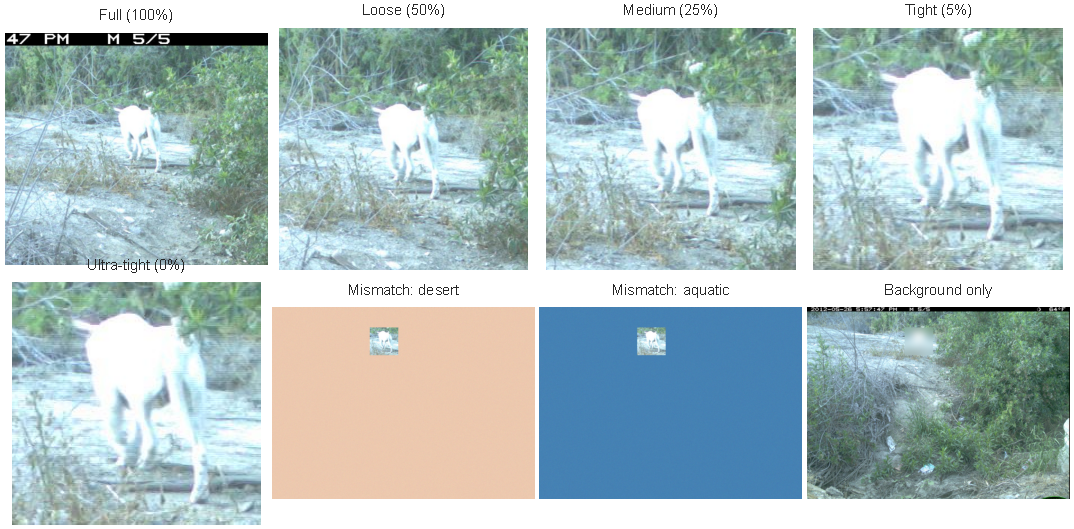
\includegraphics[width=\textwidth]{figures/fig_conditions}
\caption{The experimental conditions illustrated on one sample. Top: Experiment~1, crops that keep 100\%, 50\%, 25\%, 5\% and 0\% of the box size as margin. Bottom: Experiment~2 (animal pasted at the same position on a synthetic desert or aquatic background) and Experiment~4 (animal blurred, habitat kept).}
\label{fig:conditions}
\end{figure*}

\subsection{Models and zero-shot protocol}
We evaluate CLIP ViT-B/32 (\ParamsVB{}\,M parameters, $\PatchVB{}\times\PatchVB{}$ patches), CLIP ViT-L/14 (\ParamsVL{}\,M, $\PatchVL{}\times\PatchVL{}$) with the OpenAI weights, and BioCLIP (\ParamsBio{}\,M, ViT-B backbone with $\PatchBio{}\times\PatchBio{}$ patches) from the \texttt{imageomics/bioclip} release, all through OpenCLIP~\cite{ilharco2021} version \OpenCLIPVer{}. BioCLIP therefore differs from ViT-B/32 in patch size and training data, which matters for the interpretation in Sec.~\ref{sec:discussion}. No model is trained or fine-tuned. Each model uses its own preprocessing (bicubic resize of the shorter side to 224 pixels followed by a centre crop) and tokenizer. For a prompt template, the 16 class names (underscores replaced by spaces) are embedded; the prediction is the class with the highest cosine similarity, and the confidence is the softmax probability of that class computed from the similarities scaled by the model's learned temperature.

\subsection{Activation functions}
The OpenAI CLIP weights were trained with the QuickGELU activation $x\,\sigma(1.702x)$, an approximation of the GELU~\cite{hendrycks2016}. Recent OpenCLIP versions instantiate the architectures named \texttt{ViT-B-32} and \texttt{ViT-L-14} with the exact GELU unless QuickGELU is requested, and only emit a warning; BioCLIP's released configuration uses the exact GELU. Because this silently changes the network, we evaluate every model with both activations by replacing all MLP activation layers of the vision and text towers, without retraining: \textbf{QuickGELU} (primary, the activation of the OpenAI weights) and \textbf{GELU}. We verified that the swapped models reproduce independently constructed models to within $1.2\times10^{-7}$ in embedding values. In a separate sweep, SiLU and ReLU collapse all three models to \mbox{2.6--9.4\%} accuracy (3--7 of 16 classes predicted), so they are not used further.

\subsection{Experiments}
\textbf{Experiment 1: gradual context removal.} The image is cropped around the box $(x,y,w,h)$ with a margin of $m\in\{100,50,25,5,0\}\%$ of the box width and height on each side, clamped to the image (``full'', ``loose'', ``medium'', ``tight'', ``ultra-tight''). Prompt: ``a photo of a \emph{species}''.

\textbf{Experiment 2: context mismatch.} Baseline accuracy is measured on the original uncropped images. For every species we choose two habitats that are ecologically incompatible with it (e.g.\ no aquatic background for deer, no desert for lizard) from four synthetic backgrounds: arctic (240,248,255), desert (237,201,175), aquatic (70,130,180) and urban (169,169,169). A background is a full-size solid colour, blurred with a Gaussian of radius 12 and perturbed with Gaussian noise of standard deviation 10. The content of the animal's bounding box is pasted at its original position. This gives \NMismatch{} composites per model; the species-to-habitat assignment is released with the code and is our own choice (Sec.~\ref{sec:limits}).

\textbf{Experiment 3: prompts.} The original images are classified with four templates: neutral (``a photo of a \emph{species}''), habitat (``\ldots{} in its natural habitat''), wildlife (``a wildlife camera trap image of a \emph{species}'') and scientific (``a \emph{species} specimen'').

\textbf{Experiment 4: background only.} The bounding-box region is blurred with a Gaussian of radius 30 and the rest of the image is kept. We use $\NBg{}$ images (five per species, seed 42); chance is $1/16=6.25\%$.

\subsection{Metrics}
Let $\mathrm{Acc}$ denote accuracy in percent.
\begin{align}
\mathrm{CDS} &= \frac{\mathrm{Acc}_\text{full}-\mathrm{Acc}_\text{UT}}{\mathrm{Acc}_\text{full}}\times 100, \\
\mathrm{CR} &= \frac{\mathrm{Acc}_\text{mismatch}}{\mathrm{Acc}_\text{baseline}}\times 100, \\
\mathrm{PS} &= \frac{\max_i \mathrm{Acc}_i-\min_i \mathrm{Acc}_i}{\overline{\mathrm{Acc}_i}}\times 100,
\end{align}
where $\mathrm{Acc}_\text{full}$ and $\mathrm{Acc}_\text{UT}$ are the accuracies with 100\% and 0\% margin, and $i$ runs over the four prompts. A positive CDS means that context helps, a negative CDS that it hurts; CR near 100 means robustness to wrong habitats, and CR above 100 means that the composites are classified \emph{better} than the originals. Per-species CDS is defined as 0 when $\mathrm{Acc}_\text{full}=0$. Note that ``full'' denotes the 100\%-margin crop of Experiment~1 and differs from the uncropped baseline of Experiments~2 and~3.

\subsection{Statistics and implementation}
We report 95\% percentile bootstrap intervals (2{,}000 resamples of the samples, seed 42) for the headline metrics under QuickGELU. No correction for multiple comparisons is applied. All experiments ran in a notebook on one \GPUName{} with PyTorch \TorchVer{}; encoding all variants for all models and both activations takes about \RuntimeMin{} minutes.

\section{Results}
\subsection{Overview}
Table~\ref{tab:main} summarises the four experiments. Under both activations BioCLIP has the highest CDS and the lowest CR, ViT-L/14 is the most accurate model and the most prompt-stable, and ViT-B/32 has the highest PS. Bootstrap intervals (QuickGELU) show that BioCLIP's CDS (\QBioCDSLo--\QBioCDSHi\%) is clearly above that of ViT-L/14 (\QVLCDSLo--\QVLCDSHi\%), whereas the CDS of ViT-B/32 (\QVBCDSLo{} to \QVBCDSHi\%) includes zero.

\begin{table*}[t]
\caption{Main results on 16 animal classes. Acc in \%; CDS, CR and PS in \%; BG = background-only accuracy ($n{=}80$, chance $6.25\%$). QuickGELU is the primary configuration.}
\label{tab:main}
\centering\footnotesize
\setlength{\tabcolsep}{4pt}
\begin{tabular}{l rrrrrr rrrrrr}
\toprule
 & \multicolumn{6}{c}{QuickGELU (primary)} & \multicolumn{6}{c}{GELU}\\
\cmidrule(lr){2-7}\cmidrule(lr){8-13}
Model & Acc$_\text{full}$ & Acc$_\text{UT}$ & CDS & CR & PS & BG & Acc$_\text{full}$ & Acc$_\text{UT}$ & CDS & CR & PS & BG \\
\midrule
ViT-B/32 & 36.8 & 38.2 & $-$3.9 & 111 & 61.5 & 10.0 & 32.3 & 34.5 & $-$6.7 & 106 & 44.7 & 5.0 \\
ViT-L/14 & 59.2 & 53.9 & 9.1 & 85 & 25.8 & 11.2 & 65.2 & 57.5 & 11.9 & 77 & 15.5 & 11.2 \\
BioCLIP & 45.0 & 31.0 & 31.2 & 44 & 49.0 & 13.8 & 45.5 & 29.6 & 34.9 & 45 & 34.4 & 3.8 \\
\bottomrule
\end{tabular}
\end{table*}


\subsection{Experiment 1: gradual context removal}
Figure~\ref{fig:curves} shows accuracy and confidence as context is removed. The three models behave differently. For BioCLIP, accuracy is flat between full and loose crops (\QBioLvFull{} and \QBioLvLoose\%) and then falls steeply to \QBioLvUT\% at the ultra-tight crop (CDS \QBioCDS\%); its mean confidence falls only from \QBioLcFull{} to \QBioLcUT\%, so the confidence--accuracy gap at the ultra-tight crop reaches \QBioGap{} points (\GBioGap{} with GELU). ViT-L/14 degrades gracefully (\QVLLvFull{} to \QVLLvUT\%, CDS \QVLCDS\%) with a gap of \QVLGap{} points. ViT-B/32 is non-monotonic: accuracy rises from \QVBLvFull\% at full context to \QVBLvMedium\% at the medium crop and falls to \QVBLvUT\% at the ultra-tight crop, still above the full-context value, giving a slightly negative CDS (\QVBCDS\%; \GVBCDS\% with GELU). Cropping thus helps this small model somewhat, but the effect is not statistically distinguishable from zero.

\begin{figure*}[t]
\centering
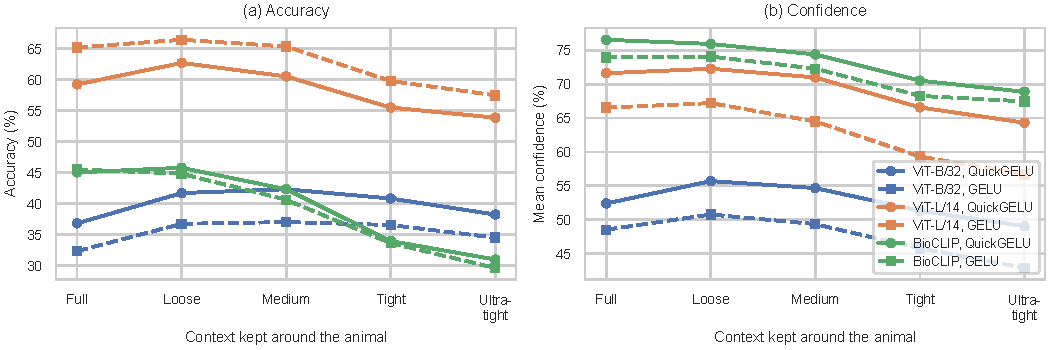
\includegraphics[width=\textwidth]{figures/fig_context_curves}
\caption{Experiment 1. Accuracy (a) and mean confidence (b) as context around the animal is removed. Solid: QuickGELU; dashed: GELU.}
\label{fig:curves}
\end{figure*}

Per-species CDS (Table~\ref{tab:species}, Fig.~\ref{fig:species}) reveals large differences. Under QuickGELU, opossum, rodent and badger are strongly context dependent for all three models (e.g.\ opossum $80$ / $32$ / $93\%$ for ViT-B/32 / ViT-L/14 / BioCLIP); these animals are small in the frame (Table~\ref{tab:dataset}). Under GELU, BioCLIP's accuracy on opossum drops to zero without context, and ViT-B/32's CDS for rodent becomes strongly negative, so individual species values depend on the activation. Dog and cat show strongly negative CDS for the OpenAI models, i.e.\ cropping \emph{improves} their classification; at full context these animals are confused with other carnivores (Sec.~\ref{sec:errors}). ViT-B/32 has a negative CDS for \QVBNeg{} of 16 species, ViT-L/14 for \QVLNeg{}, and BioCLIP for \QBioNeg{}. Per-species estimates for badger ($n=28$) and mountain lion ($n=44$) are noisy.

\begin{figure*}[t]
\centering
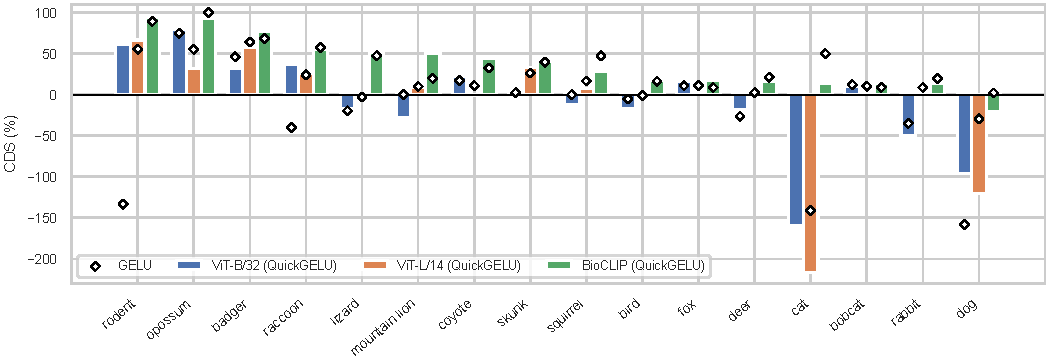
\includegraphics[width=\textwidth]{figures/fig_species_cds}
\caption{Per-species CDS (bars: QuickGELU; white diamonds: GELU), sorted by BioCLIP. CDS is 0 where full-context accuracy is 0.}
\label{fig:species}
\end{figure*}

\begin{table}[t]
\caption{Per-species CDS (\%), sorted by BioCLIP/QuickGELU; defined as 0 where Acc$_\text{full}=0$. B = ViT-B/32, L = ViT-L/14, Bio = BioCLIP.}
\label{tab:species}
\centering\footnotesize
\setlength{\tabcolsep}{3.5pt}
\begin{tabular}{l rrr rrr}
\toprule
 & \multicolumn{3}{c}{QuickGELU} & \multicolumn{3}{c}{GELU}\\
\cmidrule(lr){2-4}\cmidrule(lr){5-7}
Species & B & L & Bio & B & L & Bio \\
\midrule
rodent & 61 & 67 & 94 & $-$133 & 56 & 89 \\
opossum & 80 & 32 & 93 & 75 & 55 & 100 \\
badger & 32 & 58 & 77 & 46 & 64 & 69 \\
raccoon & 36 & 26 & 55 & $-$40 & 24 & 57 \\
lizard & $-$17 & $-$1 & 51 & $-$20 & $-$3 & 47 \\
mountain lion & $-$27 & 9 & 50 & 0 & 10 & 20 \\
coyote & 22 & $-$1 & 44 & 17 & 11 & 32 \\
skunk & 5 & 33 & 41 & 2 & 26 & 40 \\
squirrel & $-$12 & 8 & 29 & 0 & 17 & 47 \\
bird & $-$16 & 1 & 17 & $-$5 & $-$1 & 16 \\
fox & 16 & 3 & 17 & 11 & 11 & 9 \\
deer & $-$18 & 2 & 16 & $-$26 & 2 & 21 \\
cat & $-$160 & $-$217 & 14 & $-$400 & $-$141 & 50 \\
bobcat & 10 & 3 & 14 & 12 & 10 & 9 \\
rabbit & $-$50 & 4 & 13 & $-$35 & 9 & 20 \\
dog & $-$96 & $-$120 & $-$20 & $-$158 & $-$29 & 2 \\
\bottomrule
\end{tabular}
\end{table}


\subsection{Experiment 2: context mismatch}
Table~\ref{tab:mismatch} lists baseline and mismatch accuracy. BioCLIP retains only \QBioCR\% of its baseline accuracy when the animal is placed on a wrong-habitat background (CI \QBioCRLo--\QBioCRHi\%; \GBioCR\% with GELU), ViT-L/14 retains \QVLCR\% and ViT-B/32 retains all of it or more (CR \QVBCR\%, but the interval \QVBCRLo--\QVBCRHi\% includes 100). The CR above 100 for ViT-B/32 is consistent with its negative CDS: replacing the cluttered scene by a uniform background does not hurt it. Hence CR should not be read as ``robustness'' when it exceeds 100.

\begin{table*}[t]
\caption{Experiment 2: context robustness. Baseline = original image; Mismatch = animal pasted on a wrong-habitat background (accuracy over all 2,944 composites); CR = Mismatch/Baseline. Right: accuracy per synthetic habitat (arctic $n{=}1172$, desert 572, aquatic 900, urban 300). Habitat accuracies mix background and species composition (Sec.~\ref{sec:limits}).}
\label{tab:mismatch}
\centering\footnotesize
\setlength{\tabcolsep}{4pt}
\begin{tabular}{ll rrr rrrr}
\toprule
Activation & Model & Baseline & Mismatch & CR & Arctic & Desert & Aquatic & Urban \\
\midrule
QuickGELU & ViT-B/32 & 15.1 & 16.7 & 111 & 16.9 & 12.4 & 17.1 & 23.0 \\
 & ViT-L/14 & 35.9 & 30.5 & 85 & 30.9 & 22.2 & 31.8 & 40.7 \\
 & BioCLIP & 28.6 & 12.5 & 44 & 11.4 & 7.9 & 14.7 & 18.7 \\
\midrule
GELU & ViT-B/32 & 14.8 & 15.8 & 106 & 17.3 & 6.5 & 16.9 & 24.0 \\
 & ViT-L/14 & 41.8 & 32.2 & 77 & 29.3 & 28.8 & 36.6 & 37.3 \\
 & BioCLIP & 26.2 & 11.8 & 45 & 10.4 & 6.6 & 13.4 & 22.3 \\
\bottomrule
\end{tabular}
\end{table*}


Per-habitat accuracies follow an unexpected pattern. In all six model--activation combinations the urban composites yield the \emph{highest} and the desert composites the \emph{lowest} accuracy (e.g.\ ViT-L/14 with QuickGELU: urban \QVLHabUrban\%, desert \QVLHabDesert\%). This ordering should not be over-interpreted: only three species (bobcat, deer, lizard) were assigned the urban background, so habitat and species composition are confounded (Sec.~\ref{sec:limits}).

\subsection{Experiment 3: prompts}
Table~\ref{tab:prompts} shows that prompt effects depend on the model. The wildlife-specific prompt improves both OpenAI models over the neutral prompt (ViT-B/32 by \QVBPrmWild{} points, ViT-L/14 by \QVLPrmWild{} points under QuickGELU) but \emph{reduces} BioCLIP's accuracy (\QBioPrmWild{} points; \GBioPrmWild{} under GELU). The habitat prompt likewise lowers BioCLIP's accuracy (\QBioPrmHab{} points) while it raises both OpenAI models' (\QVBPrmHab{} and \QVLPrmHab{} points). The ``scientific specimen'' template is the weakest prompt only for ViT-L/14; for ViT-B/32 the neutral template is the weakest, and for BioCLIP a habitat or wildlife template is. ViT-B/32 is the most prompt-sensitive model (PS \QVBPS\%), ViT-L/14 the most stable (\QVLPS\%); BioCLIP lies in between (\QBioPS\%). PS depends strongly on the activation (Sec.~\ref{sec:activation}).

\begin{table}[t]
\caption{Experiment 3: accuracy (\%) on original images for four prompt templates, and Prompt Sensitivity PS $=(\max-\min)/\text{mean}\times100$.}
\label{tab:prompts}
\centering\footnotesize
\setlength{\tabcolsep}{3pt}
\begin{tabular}{ll rrrr r}
\toprule
Act. & Model & Neutral & Habitat & Wildlife & Scient. & PS \\
\midrule
QuickGELU & ViT-B/32 & 15.1 & 17.3 & 26.6 & 16.1 & 61.5 \\
 & ViT-L/14 & 35.9 & 44.1 & 45.2 & 34.9 & 25.8 \\
 & BioCLIP & 28.6 & 18.4 & 18.0 & 21.5 & 49.0 \\
\midrule
GELU & ViT-B/32 & 14.8 & 19.1 & 22.9 & 15.5 & 44.7 \\
 & ViT-L/14 & 41.8 & 45.4 & 45.7 & 39.1 & 15.5 \\
 & BioCLIP & 26.2 & 18.8 & 20.5 & 19.8 & 34.4 \\
\bottomrule
\end{tabular}
\end{table}


\subsection{Experiment 4: background only}
With the animal blurred, accuracy is above the 6.25\% chance level for all models under QuickGELU (Table~\ref{tab:bg}: \QVBBG{}, \QVLBG{} and \QBioBG\% for ViT-B/32, ViT-L/14 and BioCLIP), but the intervals are wide and all three include the chance level (lower bounds \QVBBGLo{}, \QVLBGLo{} and \QBioBGLo\%). Under GELU, BioCLIP (\GBioBG\%, \GBioBgn{} of 80) and ViT-B/32 (\GVBBG\%) are at or below chance. With $n=\NBg{}$ images the evidence that these models exploit habitat \emph{alone} is therefore weak and depends on the activation; it does not support a strong claim.

\begin{table}[t]
\caption{Experiment 4: accuracy (\%) from images whose animal box is blurred ($n{=}80$; chance $=6.25\%$, i.e.\ 5 of 80). Brackets: 95\% bootstrap CI.}
\label{tab:bg}
\centering\footnotesize
\setlength{\tabcolsep}{4pt}
\begin{tabular}{l rl r}
\toprule
Model & QuickGELU & 95\% CI & GELU \\
\midrule
ViT-B/32 & 10.0 (8/80) & [3.8, 16.2] & 5.0 (4/80) \\
ViT-L/14 & 11.2 (9/80) & [5.0, 18.8] & 11.2 (9/80) \\
BioCLIP & 13.8 (11/80) & [6.2, 22.5] & 3.8 (3/80) \\
\bottomrule
\end{tabular}
\end{table}


\subsection{Error structure}\label{sec:errors}
Figure~\ref{fig:confusion} shows full-context confusion matrices. The errors concentrate on a few attractor classes. For ViT-B/32 and BioCLIP, dark and low-contrast nocturnal animals (raccoon, opossum, skunk, rodent) are most often predicted as \emph{badger} (e.g.\ raccoon$\to$badger 70 times for ViT-B/32, opossum$\to$badger 71 times for BioCLIP). ViT-L/14 has a cleaner diagonal; its main errors are cat$\to$bobcat (56), fox$\to$coyote (38) and dog$\to$mountain lion or coyote (30 and 27)---visually similar carnivores. Figure~\ref{fig:qualitative} gives examples of the manipulations and of the resulting predictions: for the dog the ultra-tight crop changes ViT-L/14's prediction from bobcat to deer and BioCLIP's from cat to the correct class, while for the dark opossum frame all models fail without context.

\begin{figure*}[t]
\centering
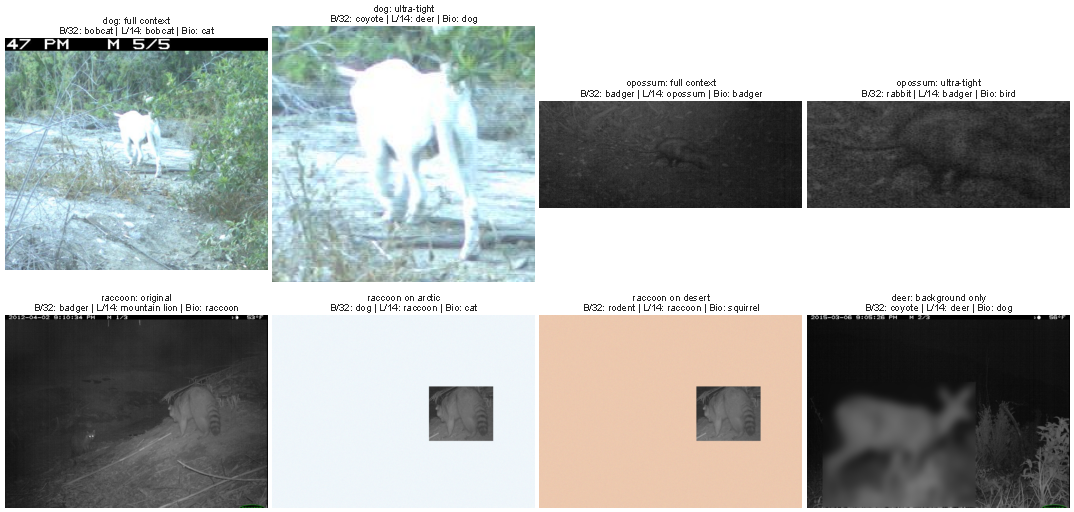
\includegraphics[width=\textwidth]{figures/fig_qualitative}
\caption{Qualitative examples (QuickGELU, first sample of each species in the sample list, not selected). Titles give the predictions of ViT-B/32, ViT-L/14 and BioCLIP. Top: dog and opossum at full context and with the ultra-tight crop. Bottom: raccoon original and on two wrong-habitat backgrounds; deer with the animal blurred.}
\label{fig:qualitative}
\end{figure*}

\begin{figure*}[t]
\centering
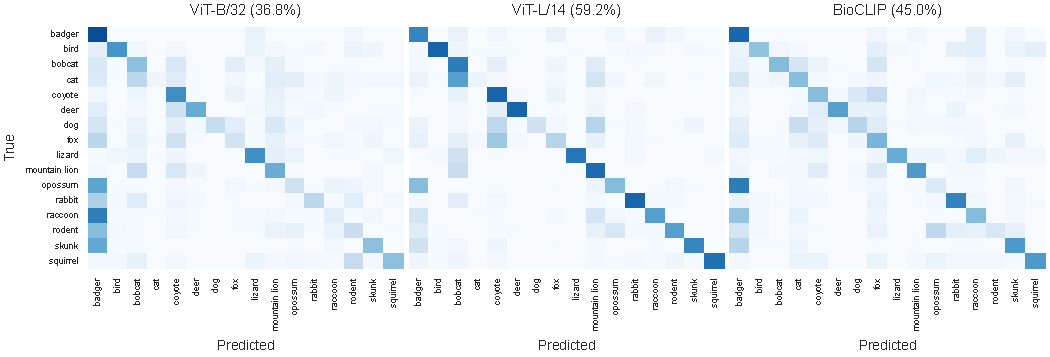
\includegraphics[width=\textwidth]{figures/fig_confusion}
\caption{Row-normalised confusion matrices at full context (QuickGELU, neutral prompt). Overall accuracy in the panel titles.}
\label{fig:confusion}
\end{figure*}

\subsection{Sensitivity to the activation function}\label{sec:activation}
Figure~\ref{fig:activation} compares the two activations. Switching from GELU to QuickGELU changes the full-context accuracy of ViT-B/32 by \DeltaVBFull{} points, of ViT-L/14 by \DeltaVLFull{} points and of BioCLIP by \DeltaBioFull{} points. The direction differs between the two OpenAI models (QuickGELU helps ViT-B/32 and hurts ViT-L/14 on this data), so the activation cannot be treated as a nuisance parameter. CDS shifts by \DeltaVBCDS{}, \DeltaVLCDS{} and \DeltaBioCDS{} points and PS by \DeltaVBPS{}, \DeltaVLPS{} and \DeltaBioPS{} points. The qualitative ordering of CDS (BioCLIP $>$ ViT-L/14 $>$ ViT-B/32) is preserved, while PS and the background-only accuracy are fragile. BioCLIP's own configuration uses GELU; QuickGELU is therefore a non-native activation for it.

\begin{figure*}[t]
\centering
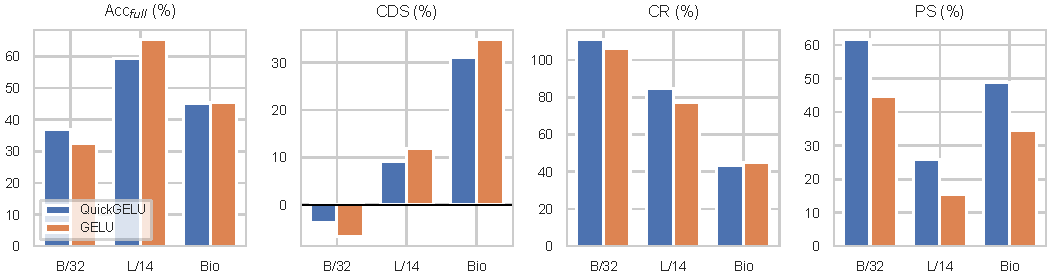
\includegraphics[width=\textwidth]{figures/fig_activation}
\caption{Effect of the activation function on full-context accuracy, CDS, CR and PS (16 classes).}
\label{fig:activation}
\end{figure*}

\subsection{Day versus night, animal size and calibration}
Roughly \NightShare\% of the samples are grayscale infrared frames. Context dependence differs strongly between frame types (Table~\ref{tab:daynight}, Fig.~\ref{fig:daynight}a). On colour frames, cropping \emph{helps} both OpenAI models (CDS \DayVBCDS{} and \DayVLCDS\%), whereas on infrared frames context helps them (CDS \NightVBCDS{} and \NightVLCDS\%); BioCLIP depends on context in both regimes, much more at night (\DayBioCDS{} versus \NightBioCDS\%). The aggregated CDS therefore averages two different regimes. Possible reasons---low-resolution, low-contrast crops of small night animals, or a different species and camera mix at night---were not tested here. Across species, CDS is only weakly related to the animal's relative size (Spearman $\rho=$ \RhoVB{}, \RhoVL{}, \RhoBio{} for the three models; none significant, $p\geq\PvalVL{}$, $n=16$ species).

\begin{table}[t]
\caption{Context dependence by frame type (QuickGELU, Experiment 1). Colour frames are daytime; grayscale frames are infrared night images.}
\label{tab:daynight}
\centering\footnotesize
\setlength{\tabcolsep}{4pt}
\begin{tabular}{ll r rrr}
\toprule
Model & Frames & $n$ & Acc$_\text{full}$ & Acc$_\text{UT}$ & CDS \\
\midrule
ViT-B/32 & Colour & 632 & 51.9 & 61.1 & $-$17.7 \\
 & Infrared & 840 & 25.5 & 21.1 & 17.3 \\
\midrule
ViT-L/14 & Colour & 632 & 69.2 & 74.2 & $-$7.3 \\
 & Infrared & 840 & 51.8 & 38.6 & 25.5 \\
\midrule
BioCLIP & Colour & 632 & 54.9 & 44.5 & 19.0 \\
 & Infrared & 840 & 37.6 & 20.8 & 44.6 \\
\bottomrule
\end{tabular}
\end{table}


Calibration differs sharply. At the ultra-tight crop BioCLIP's mean confidence is \CalConfUTBio\% against an accuracy of \QBioUT\% (expected calibration error \EceUTBio\%), whereas ViT-B/32 and ViT-L/14 have errors of \EceUTVB{} and \EceUTVL\%. Confidence thresholds would therefore filter BioCLIP's context-stripped errors poorly.

\subsection{The control class and the label set}
The initial design of this study included ``car'' as a non-animal control that should have no habitat dependence. In practice, car boxes fill the frame: for \CarCrop\% of car samples the full-context crop is already the whole image (Fig.~\ref{fig:daynight}b), so all crop levels are the same picture and CDS is zero by construction; BioCLIP additionally classifies no car correctly. A zero CDS for ``car'' thus cannot validate the metric, and the class is excluded from our main analysis. Deer is affected to a smaller degree (\DeerCrop\% of full crops equal the whole image). Table~\ref{tab:17class} shows that removing car and changing the activation shifts accuracy by several points but leaves the main conclusions intact.

\begin{figure*}[t]
\centering
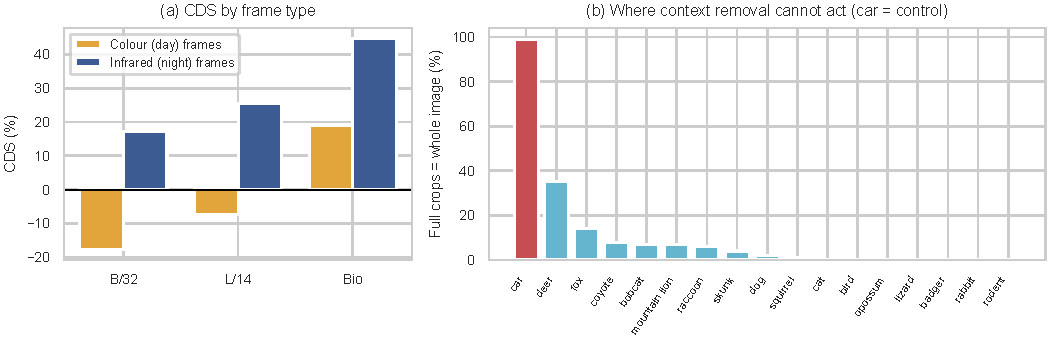
\includegraphics[width=\textwidth]{figures/fig_daynight_coverage}
\caption{(a) CDS on colour (day) and infrared (night) frames, QuickGELU. (b) Share of full-context crops that already cover the entire image; car boxes fill the frame, so CDS is zero by construction.}
\label{fig:daynight}
\end{figure*}

\begin{table*}[t]
\caption{Sensitivity to the label set and activation. 17 classes include the non-animal control `car'. 17c-GELU: plain-GELU build (the default of recent open\_clip for the OpenAI weights); 17c-QG: QuickGELU for the OpenAI models, native GELU for BioCLIP; 16c-QG: our primary configuration. Samples are identical across rows except for the removed car boxes.}
\label{tab:17class}
\centering\footnotesize
\setlength{\tabcolsep}{4pt}
\begin{tabular}{l rrr rrr rrr}
\toprule
 & \multicolumn{3}{c}{17c-GELU} & \multicolumn{3}{c}{17c-QG} & \multicolumn{3}{c}{16c-QG (primary)}\\
\cmidrule(lr){2-4}\cmidrule(lr){5-7}\cmidrule(lr){8-10}
Model & Acc$_\text{full}$ & CDS & CR & Acc$_\text{full}$ & CDS & CR & Acc$_\text{full}$ & CDS & CR \\
\midrule
ViT-B/32 & 34.5 & $-$6.1 & 105 & 38.7 & $-$3.3 & 108 & 36.8 & $-$3.9 & 111 \\
ViT-L/14 & 63.0 & 11.5 & 78 & 55.9 & 9.0 & 85 & 59.2 & 9.1 & 85 \\
BioCLIP & 42.6 & 34.8 & 45 & 42.6 & 34.8 & 45 & 45.0 & 31.2 & 44 \\
\bottomrule
\end{tabular}
\end{table*}


\section{Discussion}\label{sec:discussion}
\textbf{What the experiments show.} Context contributes substantially to the zero-shot accuracy of BioCLIP and, to a smaller extent, of ViT-L/14, but not measurably to that of ViT-B/32, which is helped slightly by removing clutter. BioCLIP's high CDS, low CR and high overconfidence together mean that it is the model most likely to fail silently when the background changes. A plausible explanation is that its training images (naturalist photographs) show animals in characteristic habitats, and that fine-tuning strengthens species--habitat associations. We stress that our experiment does not test this explanation: BioCLIP differs from ViT-B/32 in patch size and training data at the same time, so ``domain specialisation'' is not isolated as the cause.

\textbf{Context is not uniformly harmful or helpful.} The sign of CDS for the OpenAI models flips between colour and infrared frames and between species. A single dataset-wide CDS hides this structure; we recommend reporting it by frame type and species, together with intervals.

\textbf{Practical implications.} For small models and daytime imagery, detecting the animal and classifying the crop is a reasonable choice, in line with detector-first pipelines~\cite{beery2019}; for infrared imagery the benefit is not guaranteed and should be checked. Prompts should be tuned per model: a wildlife-specific prompt helps the OpenAI models and hurts BioCLIP. Confidence scores of BioCLIP should be recalibrated before they are used for filtering.

\textbf{Reproducibility.} The result depends on details that are easy to overlook: the activation function of the OpenAI weights (Sec.~\ref{sec:activation}), the label set including non-animal classes, and the sampling unit (box versus image). We therefore report two activations and the 17-class variant, and release all code.

\subsection{Limitations}\label{sec:limits}
(i) The synthetic backgrounds are solid colours with noise; the pasted box keeps its original local surroundings, so ``mismatch'' removes only the global habitat. The OpenCLIP centre crop also removes the left and right image margins in Experiments~2--4. (ii) The species-to-habitat assignment is our own and is confounded with species composition in the per-habitat results. (iii) Sampling is per box, so a few images appear more than once, and the badger and mountain-lion samples are small and come from few cameras. (iv) One region (southern California), three models and no mechanistic analysis; the explanations offered above are hypotheses. (v) Bootstrap intervals treat samples as independent, although boxes from one camera sequence are correlated; they are therefore optimistic. (vi) Background-only results rest on 80 images. (vii) Night/day is inferred from grayscale frames, not from time stamps.

\section{Conclusion}
We introduced a protocol and three metrics to measure how much zero-shot VLMs rely on habitat context when classifying camera-trap animals. On 16 species from Caltech Camera Traps, BioCLIP is the most context dependent and least robust model, ViT-L/14 is intermediate, and ViT-B/32 shows no measurable benefit from context. The results are sensitive to implementation details---the activation function, the frame type and the choice of control class---which should be reported in future studies. Evaluating more models, additional datasets, photorealistic background synthesis and mechanistic explanations remain future work.

\section*{Reproducibility statement}
All figures, tables and numbers in this paper are generated from the released notebooks and scripts: one notebook runs the complete experiment (EDA, sampling, four experiments, both activations), a second notebook produces the tables, figures and benchmark comparisons. Per-image predictions, the sample list and the species-to-habitat assignment are included.

\begin{thebibliography}{00}
\bibitem{swanson2015} A.~Swanson, M.~Kosmala, C.~Lintott, R.~Simpson, A.~Smith, and C.~Packer, ``Snapshot Serengeti, high-frequency annotated camera trap images of 40 mammalian species in an African savanna,'' \emph{Scientific Data}, vol.~2, 150026, 2015.
\bibitem{burton2015} A.~C. Burton \emph{et al.}, ``Wildlife camera trapping: a review and recommendations for linking surveys to ecological processes,'' \emph{J. Appl. Ecol.}, vol.~52, no.~3, pp.~675--685, 2015.
\bibitem{norouzzadeh2018} M.~S. Norouzzadeh \emph{et al.}, ``Automatically identifying, counting, and describing wild animals in camera-trap images with deep learning,'' \emph{Proc. Natl. Acad. Sci. USA}, vol.~115, no.~25, pp.~E5716--E5725, 2018.
\bibitem{tabak2019} M.~A. Tabak \emph{et al.}, ``Machine learning to classify animals in camera trap images: Applications in ecology,'' \emph{Methods Ecol. Evol.}, vol.~10, no.~4, pp.~585--590, 2019.
\bibitem{willi2019} M.~Willi \emph{et al.}, ``Identifying animal species in camera trap images using deep learning and citizen science,'' \emph{Methods Ecol. Evol.}, vol.~10, no.~1, pp.~80--91, 2019.
\bibitem{beery2018} S.~Beery, G.~Van~Horn, and P.~Perona, ``Recognition in terra incognita,'' in \emph{Proc. ECCV}, 2018, pp.~456--473.
\bibitem{schneider2020} S.~Schneider, S.~Greenberg, G.~W. Taylor, and S.~C. Kremer, ``Three critical factors affecting automated image species recognition performance for camera traps,'' \emph{Ecol. Evol.}, vol.~10, no.~7, pp.~3503--3517, 2020.
\bibitem{beery2019} S.~Beery, D.~Morris, and S.~Yang, ``Efficient pipeline for camera trap image review,'' arXiv:1907.06772, 2019.
\bibitem{radford2021} A.~Radford \emph{et al.}, ``Learning transferable visual models from natural language supervision,'' in \emph{Proc. ICML}, PMLR 139, 2021, pp.~8748--8763.
\bibitem{stevens2024} S.~Stevens \emph{et al.}, ``BioCLIP: A vision foundation model for the tree of life,'' in \emph{Proc. IEEE/CVF CVPR}, 2024, pp.~19412--19424.
\bibitem{ilharco2021} G.~Ilharco \emph{et al.}, ``OpenCLIP,'' Zenodo, 2021, doi:10.5281/zenodo.5143773.
\bibitem{dosovitskiy2021} A.~Dosovitskiy \emph{et al.}, ``An image is worth 16x16 words: Transformers for image recognition at scale,'' in \emph{Proc. ICLR}, 2021.
\bibitem{hendrycks2016} D.~Hendrycks and K.~Gimpel, ``Gaussian error linear units (GELUs),'' arXiv:1606.08415, 2016.
\bibitem{geirhos2020} R.~Geirhos \emph{et al.}, ``Shortcut learning in deep neural networks,'' \emph{Nat. Mach. Intell.}, vol.~2, pp.~665--673, 2020.
\bibitem{geirhos2019} R.~Geirhos \emph{et al.}, ``ImageNet-trained CNNs are biased towards texture; increasing shape bias improves accuracy and robustness,'' in \emph{Proc. ICLR}, 2019.
\bibitem{xiao2021} K.~Xiao, L.~Engstrom, A.~Ilyas, and A.~Madry, ``Noise or signal: The role of image backgrounds in object recognition,'' in \emph{Proc. ICLR}, 2021.
\bibitem{singh2020} K.~K. Singh \emph{et al.}, ``Don't judge an object by its context: Learning to overcome contextual bias,'' in \emph{Proc. IEEE/CVF CVPR}, 2020, pp.~11070--11078.
\bibitem{zhou2022} K.~Zhou, J.~Yang, C.~C. Loy, and Z.~Liu, ``Learning to prompt for vision-language models,'' \emph{Int. J. Comput. Vis.}, vol.~130, no.~9, pp.~2337--2348, 2022.
\bibitem{lila} ``LILA BC: Labeled Information Library of Alexandria: Biology and Conservation,'' \url{https://lila.science}.
\end{thebibliography}

\end{document}
